\documentclass{article}

\usepackage[a4paper, total={6.5in, 11in}]{geometry}
\usepackage{graphicx}
\graphicspath{{titech/CSC.T527.FaultTolerantDistributedAlgorithm/}}

\usepackage{latex/common}

\title{FTDA 2021 - Homework 4}
\author{Sixue Wang\\Tokyo Institute of Technology}

\begin{document}

\maketitle

\section*{Question 1}
(1,1,1) is the only satisfactory configuration. In order to decide in the first asynchronous round, $s_i=1$, so the majority of proposed values should be 1. On the other hand, 1 process could crash, so all of them should be 1.

\section*{Question 2}
(0,0,0) is the only satisfactory configuration. If there is one proposed value is 1, then there must be a situation which some processes receive 1, then no matter what the majority is, the estimated value will be updated to 1, so it could not decide in the second round. On the other hand, if all of them are 0, the estimated value will be keep as 0.

\section*{Question 3}
If there are two proposed values equal to 1, then they are guaranteed to decide by round 3. In the first round, no estimated values will be updated to 0 because 0 is not the majority and $s_i=1$. So after the first round, all estimated vlaues equal to 1. They keep 1 at the second round because 1 is the majority. At last, they decide on round 3.

\section*{Question 4}
If no processes crash and there are two proposed values equal to 0, it's possible to excute infinitely.
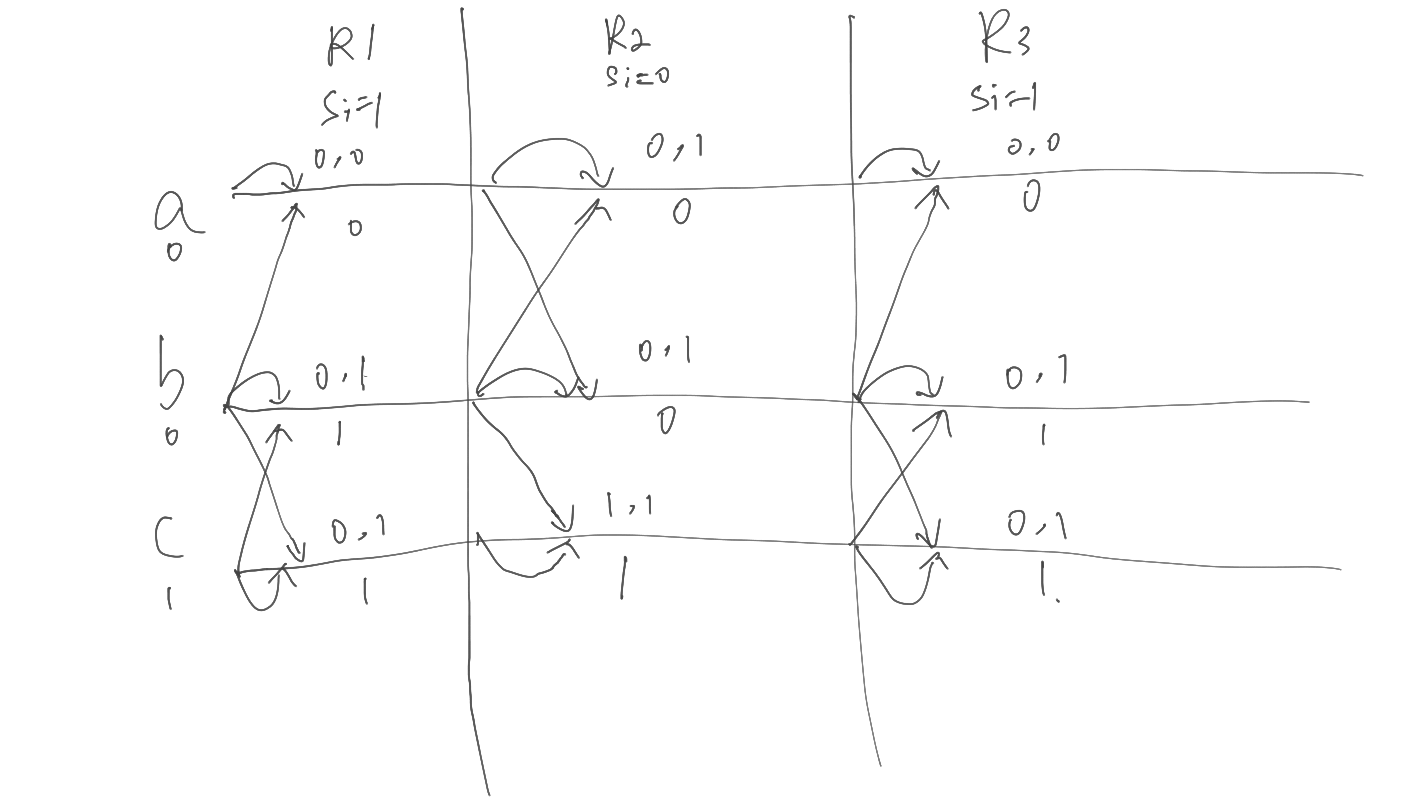
\includegraphics[width=\textwidth]{hw4_1}
On odd rounds, receiving messages according to the first round; On even rounds, receiving messages according to the second round.
We guarantee that one process receive the majority which equals to $1-s_i$ (so it cannot decide) and other two processes don't receive the majority and uses $s_i$.


\section*{Question 5}
Suppose $n=2m-1$, if not, let one process crash at the begining. $m$ processess propose 0 and $m-1$ processess propose 1 initially.
In ith round, there are $m$ estimated values equal to $1-s_i$ and $m-1$ estimated values equal to $s_i$. Let $m-1$ processes receive $1-s_i$ $m$ time, and let $m$ processes receive $s_i$ once at least. As the result, $m-1$ processes keep $1-s_i$ again, and one more process estimate with $s_i$.


\section*{Question 6}
The answer with regard to validity is yes. If all proposed values are the same, they will decide the this value finally. If 0 and 1 are both proposed, then deciding anyone is ok.

The answer with regard to agreement is also yes. Suppose one process decides $v$, there are at least $n/2$ estimated value equal $v$. There are two possible situation: 1) the process receives the majority value equals $v$; 2) the process cannot receive a majority value, it will update estimated value with $s_i=v$. As the result all processes estimate the same value $v$.

\end{document}
